\lstinputlisting[language=bash,basicstyle=\small]{python_codes/fieldstone_35/keywords}

\begin{center}
Code at \url{https://github.com/cedrict/fieldstone/tree/master/python_codes/fieldstone_35}
\end{center}

\par\noindent\rule{\textwidth}{0.4pt}
%%%%%%%%%%%%%%%%%%%%%%%%%%%%%%%%%%%%%%%%%%%%%%%%%%%%%%%%%%%%%%%%%%%%%%%%%%%%%%%%%%%%%%%%%%%%

The domain is an annulus of inner radius $R_1$ and outer radius $R_2$. Gravity is radial 
and has norm 1. 
The velocity, pressure and density fields have been derived in Section~\ref{ss:anconv2}:
\begin{eqnarray}
\upnu_r (r,\theta)&=& -\frac{1}{r} (
{ ar^4}
+{ br^3}
+{c r^2}
+ {dr}
+{e}
)k\sin(k\theta)\\
\upnu_\theta(r,\theta)&=& -(4ar^3+3br^2 +2cr + d ) \cos(k\theta) \\
p(r,\theta) &= &
\frac{1}{k}\sin(k\theta) 
\left[
2(k^2-16)ar^2
+(k^2-9)br
-k^2c
+(1-k^2)\frac{d}{r}
-2k^2\frac{e}{r^2}
\right] \\
\rho(r,\theta)&=&\frac{\sin(k\theta)}{k}
\frac{
A{ ar^4}+
B{ br^3}+
C{c r^2} +
D {dr}+
E{e}
}{r^3}
\end{eqnarray}
with
\begin{eqnarray}
a &=& 1  \nn\\
b &=& -2R_1-2R_2 \nn\\
c &=& R_1^2+R_2^2+4R_1R_2 \nn\\
d &=& -2R_1R_2^2-2R_1^2R_2 \nn\\
e &=& R_1^2R_2^2 \nn\\
A &=& (k^2-4)(k^2-16)\nn \\
B &=& k^4-10k^2+9\nn    \\
C &=& k^2(k^2-4)  \nn    \\
D &=& (k^2-1)(k^2-1) \nn     \\
E &=& k^2(k^2-4) \nn
\end{eqnarray}

boundary conditions are then no-slip on the inner and outer boundaries.

\begin{center}
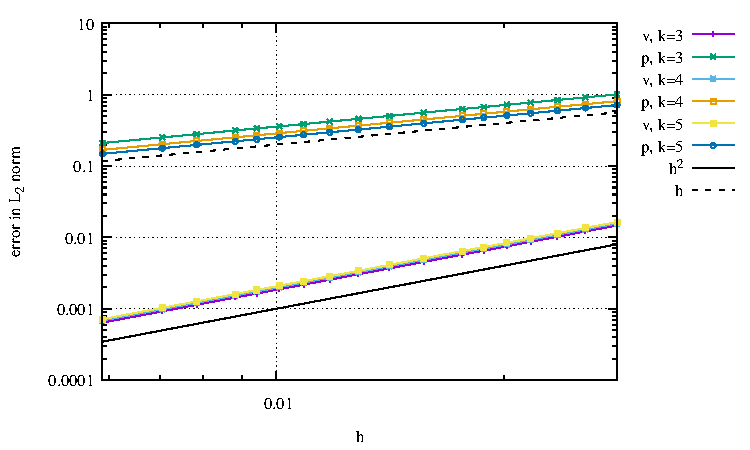
\includegraphics[width=8cm]{python_codes/fieldstone_35/results/errors}
\end{center}

\newpage
\begin{center}
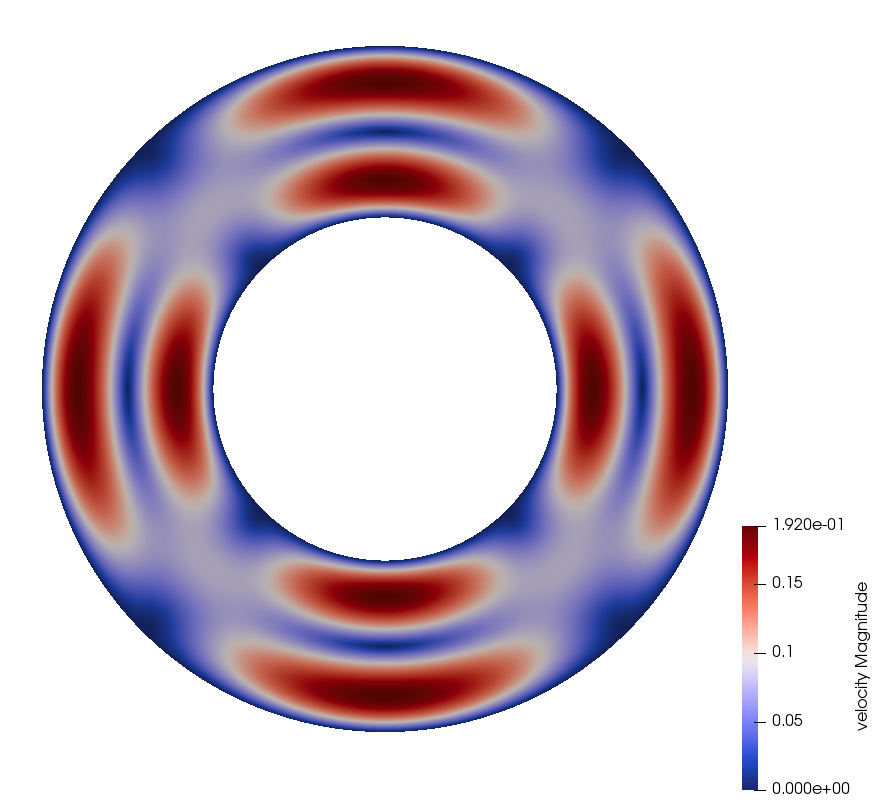
\includegraphics[width=4cm]{python_codes/fieldstone_35/results/vel_k2}
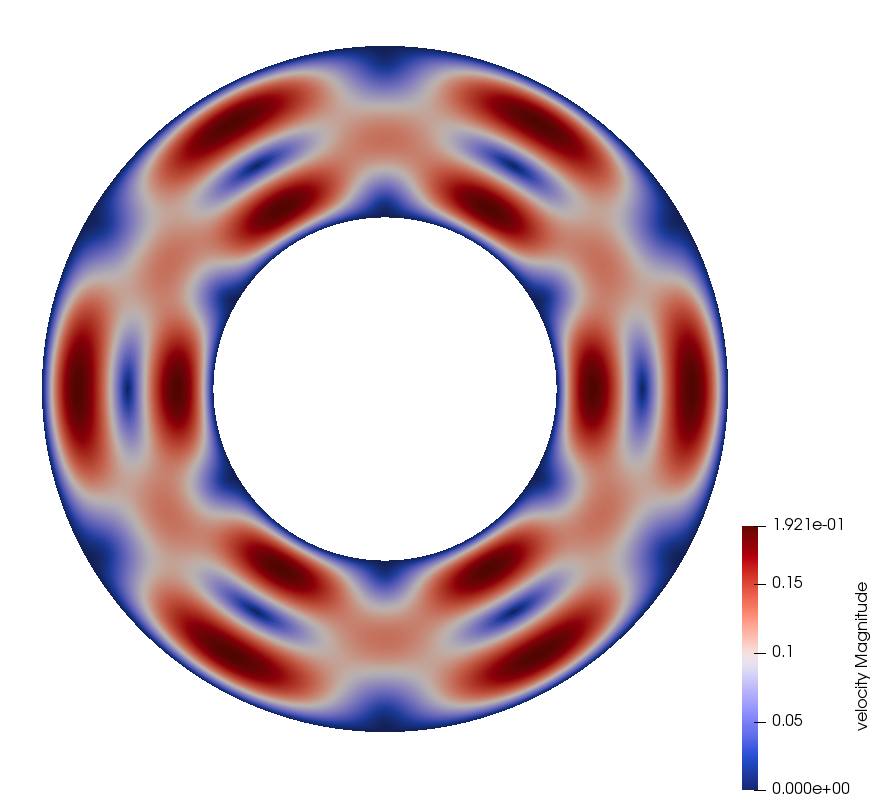
\includegraphics[width=4cm]{python_codes/fieldstone_35/results/vel_k3}
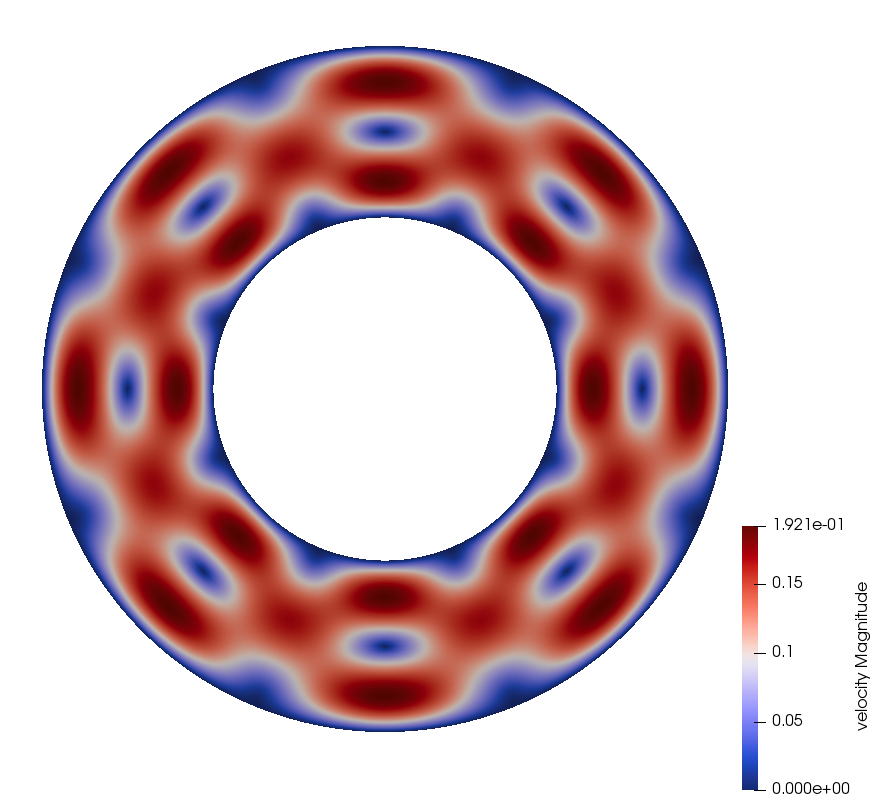
\includegraphics[width=4cm]{python_codes/fieldstone_35/results/vel_k4}
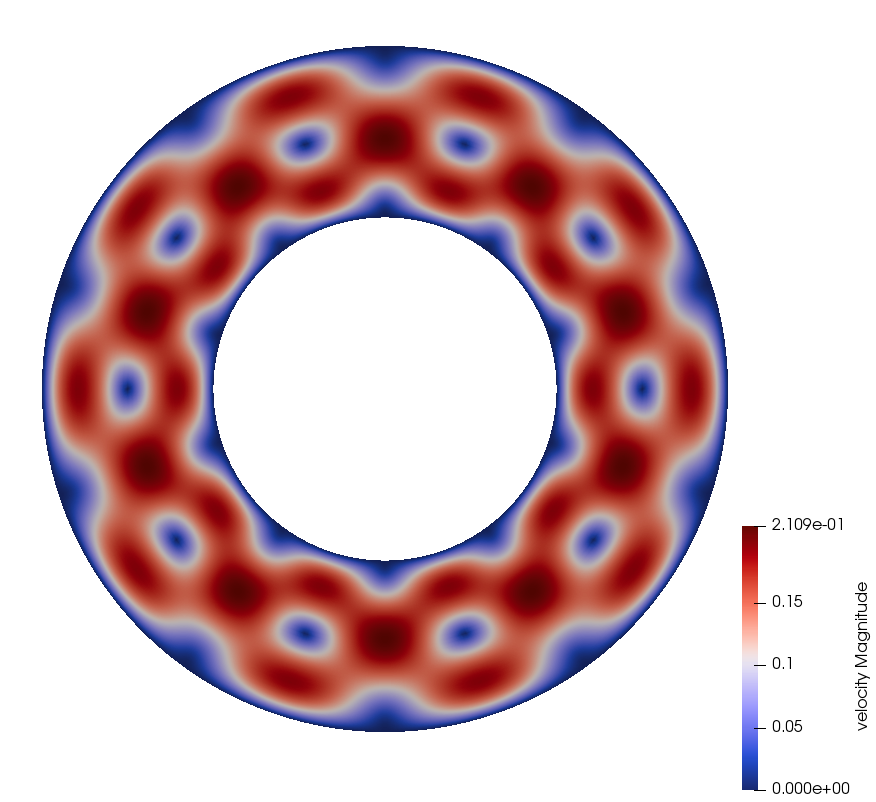
\includegraphics[width=4cm]{python_codes/fieldstone_35/results/vel_k5}\\
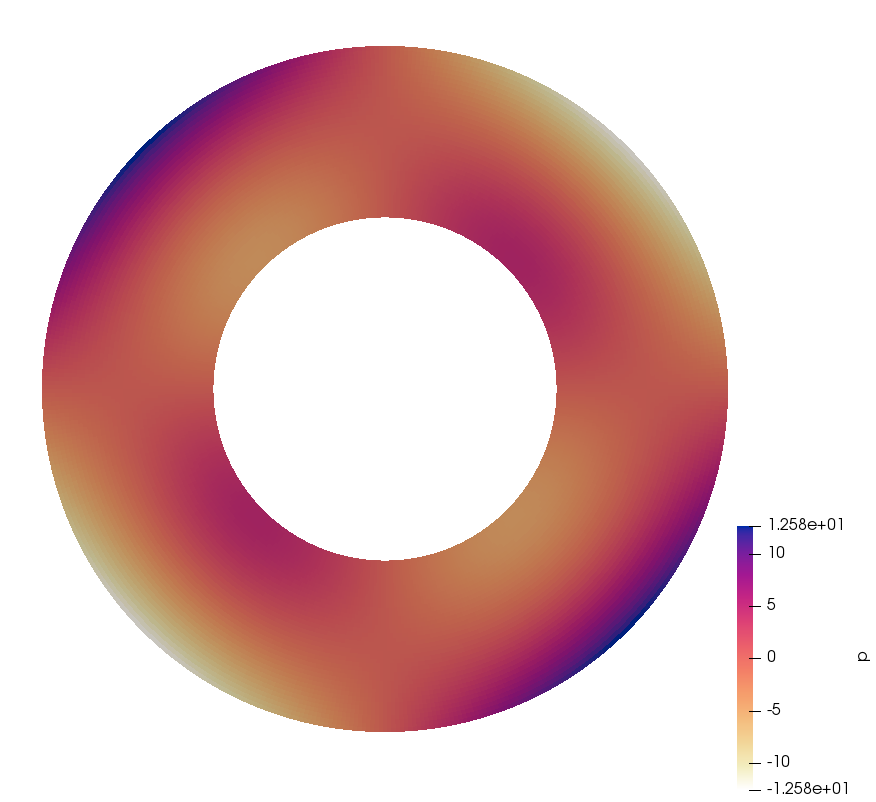
\includegraphics[width=4cm]{python_codes/fieldstone_35/results/p_k2}
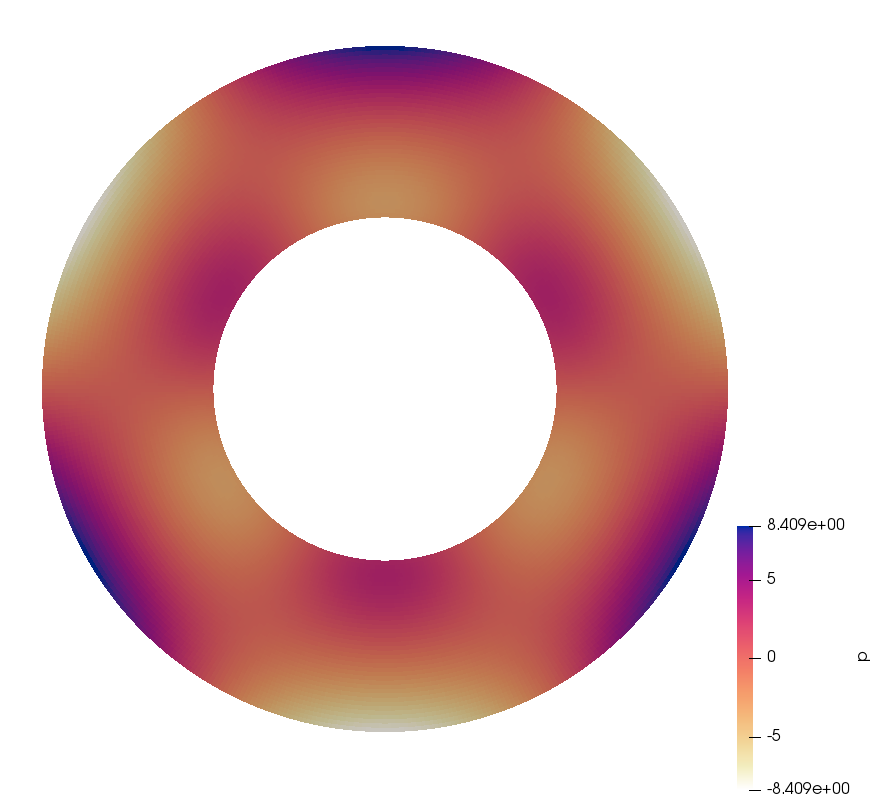
\includegraphics[width=4cm]{python_codes/fieldstone_35/results/p_k3}
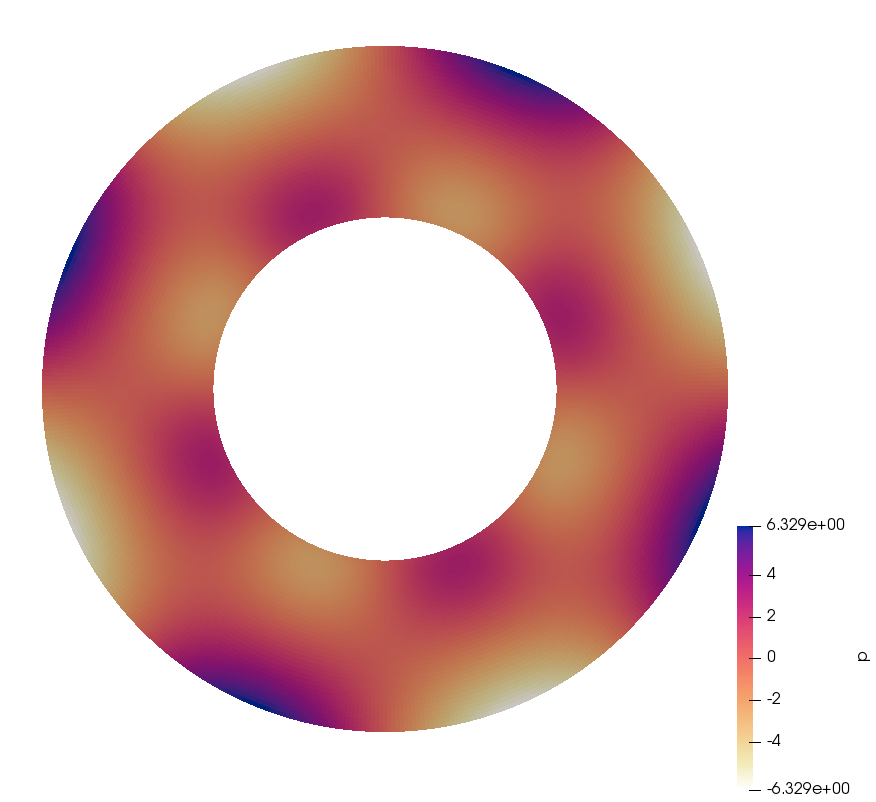
\includegraphics[width=4cm]{python_codes/fieldstone_35/results/p_k4}
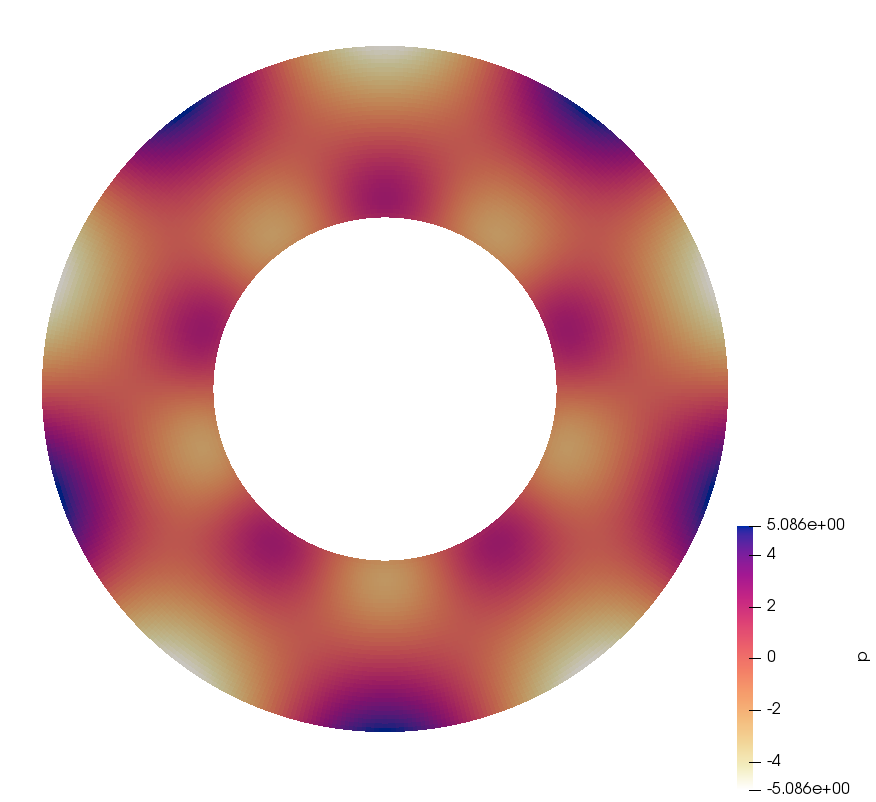
\includegraphics[width=4cm]{python_codes/fieldstone_35/results/p_k5}\\
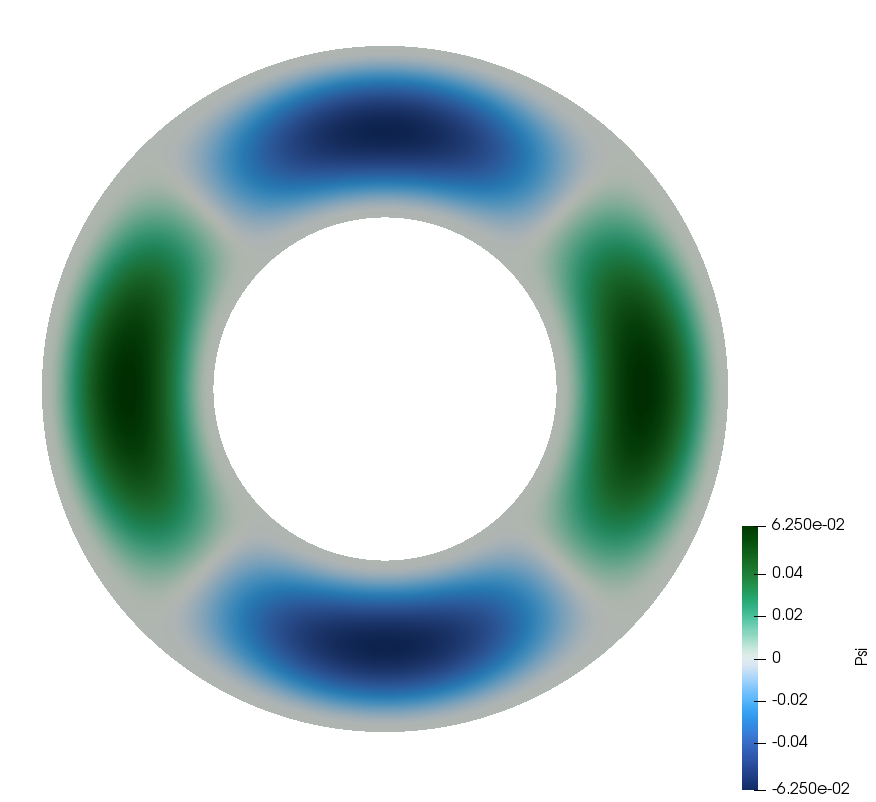
\includegraphics[width=4cm]{python_codes/fieldstone_35/results/psi_k2}
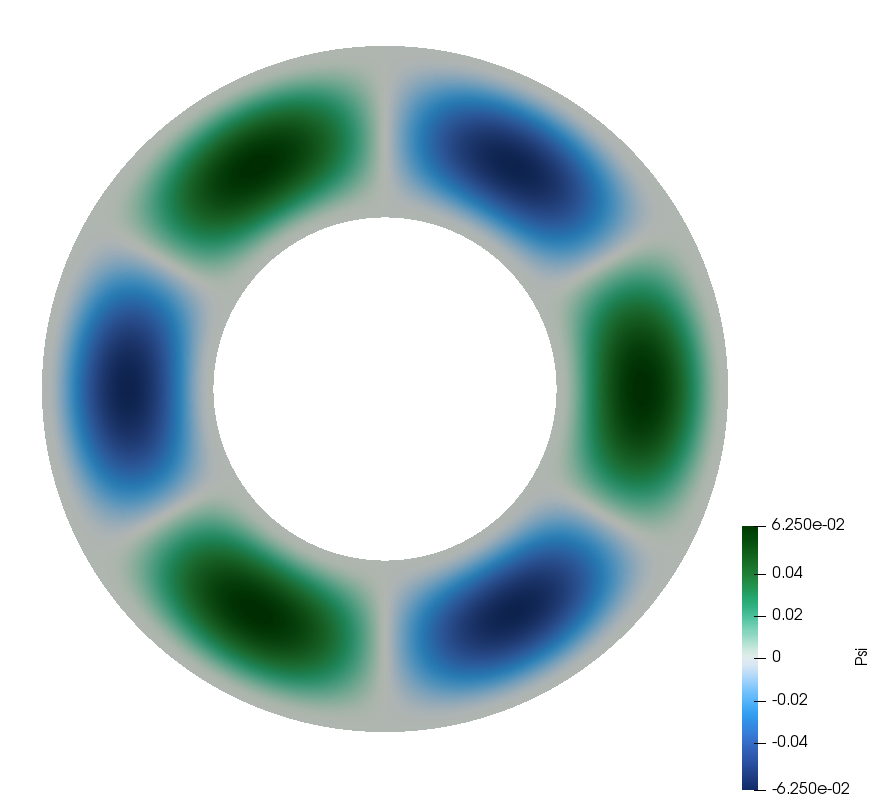
\includegraphics[width=4cm]{python_codes/fieldstone_35/results/psi_k3}
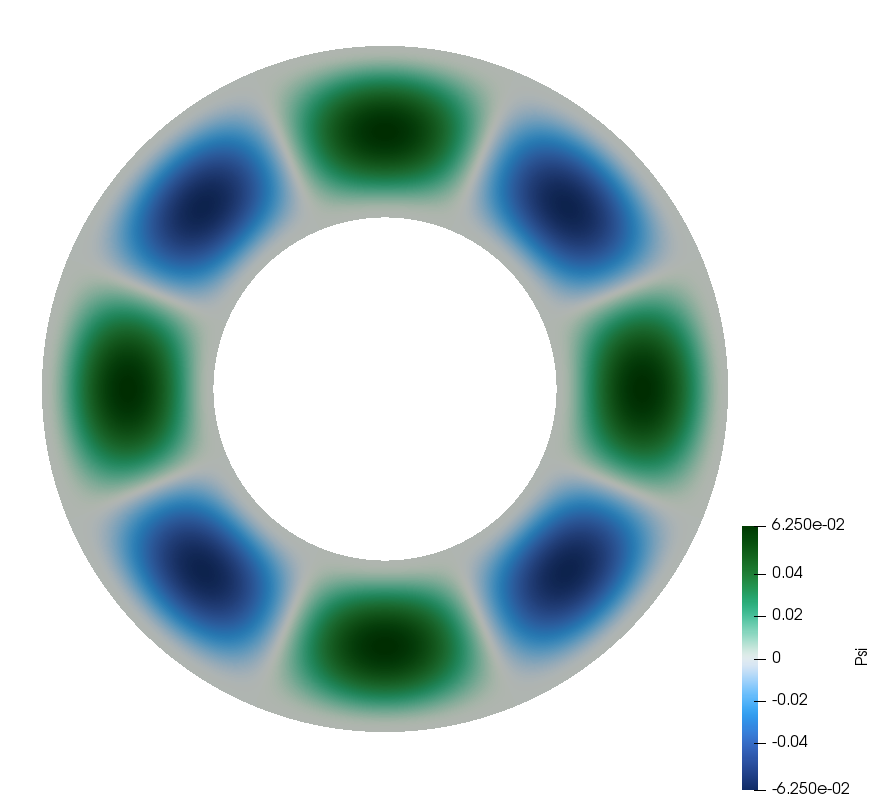
\includegraphics[width=4cm]{python_codes/fieldstone_35/results/psi_k4}
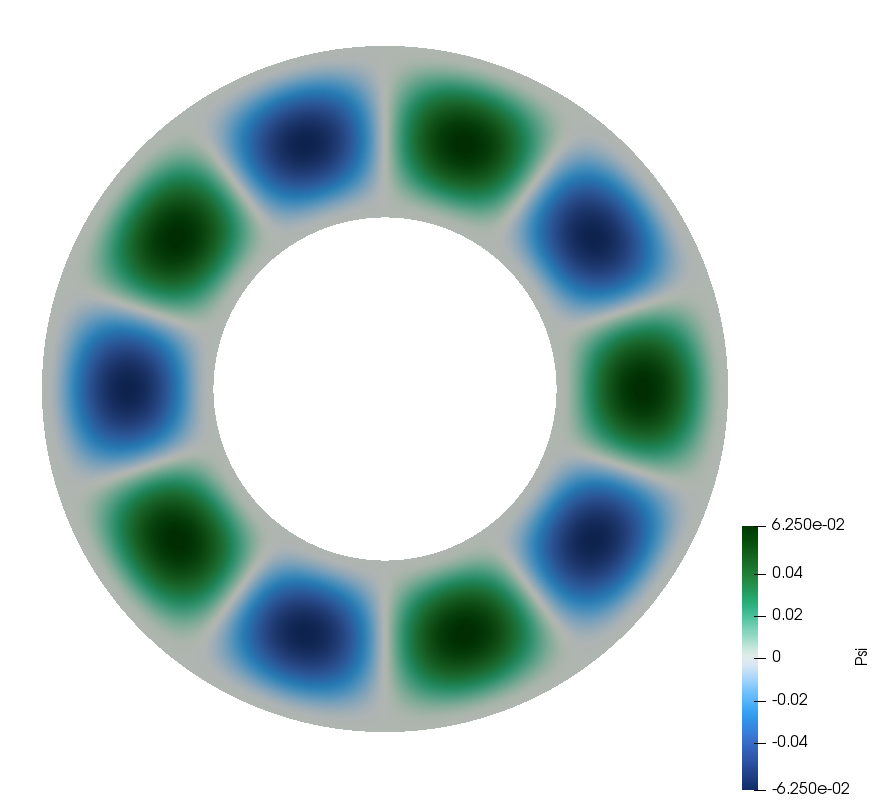
\includegraphics[width=4cm]{python_codes/fieldstone_35/results/psi_k5}\\
{\captionfont From left to right: $k=2,3,4,5$}
\end{center}



\begin{center}
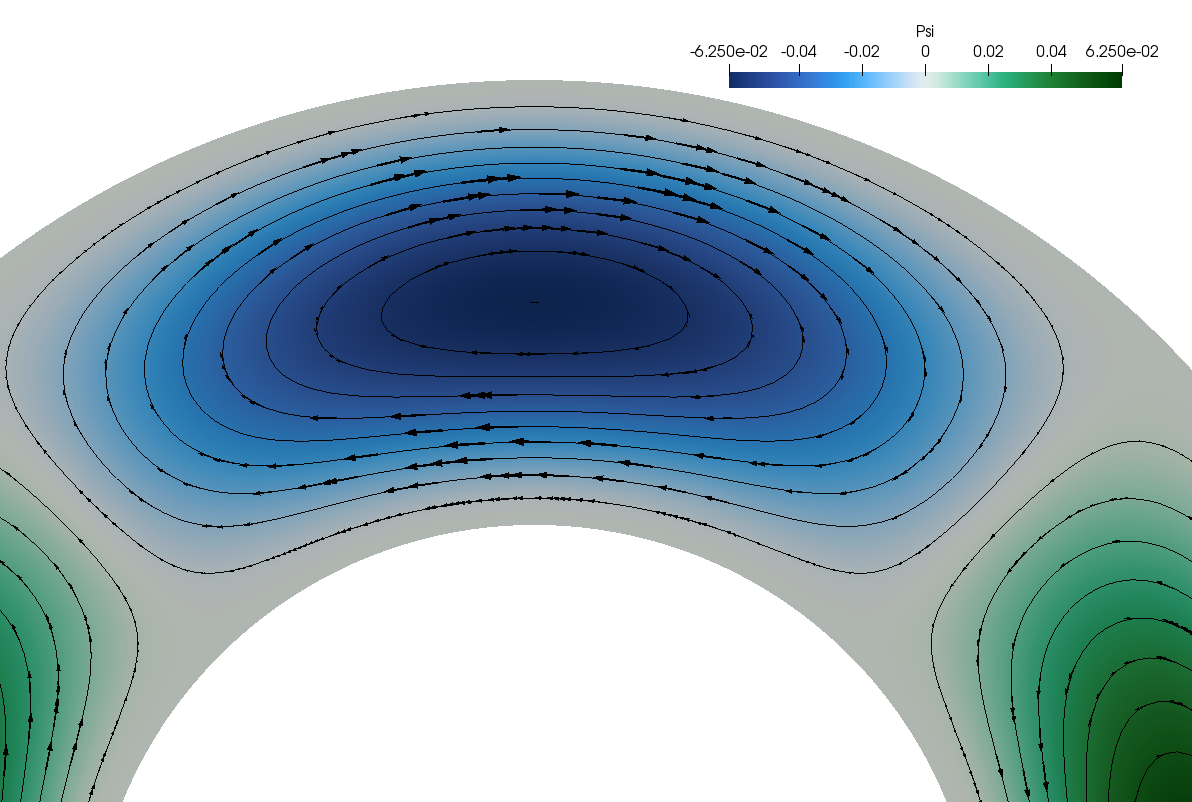
\includegraphics[width=7.3cm]{python_codes/fieldstone_35/results/iso_k2}
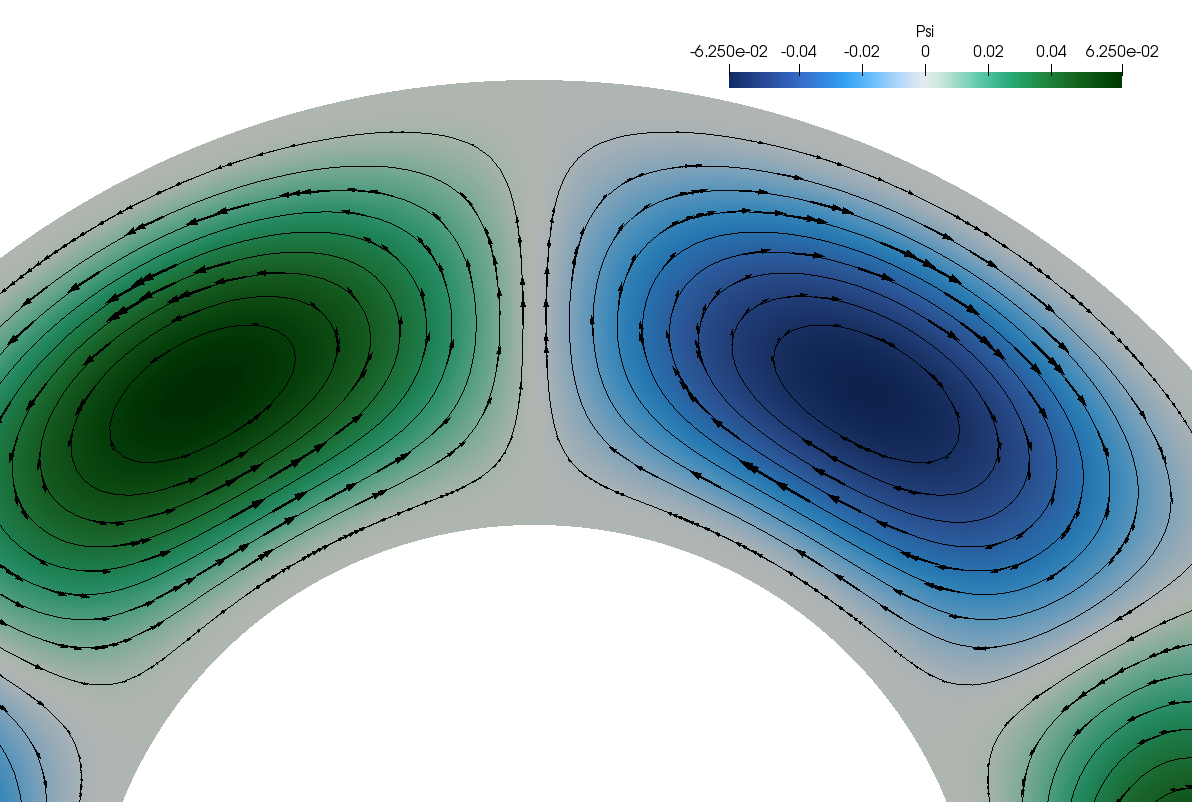
\includegraphics[width=7.3cm]{python_codes/fieldstone_35/results/iso_k3}\\
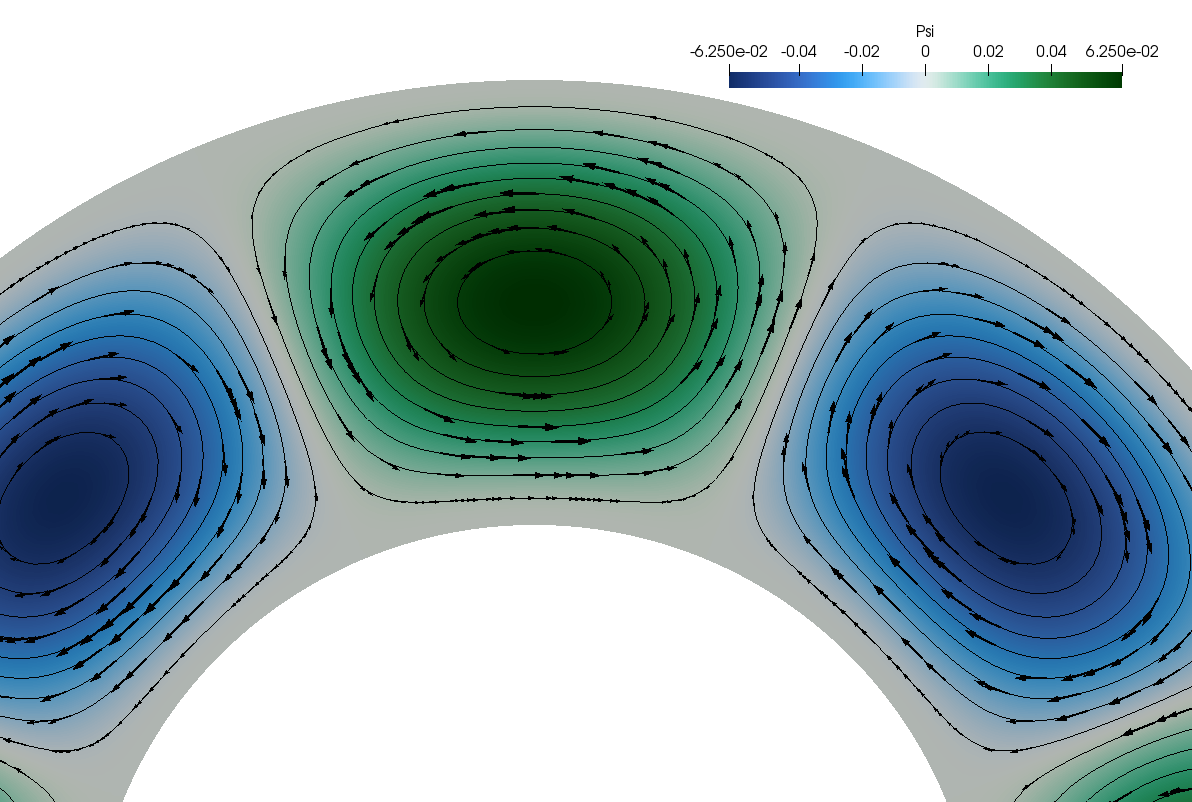
\includegraphics[width=7.3cm]{python_codes/fieldstone_35/results/iso_k4}
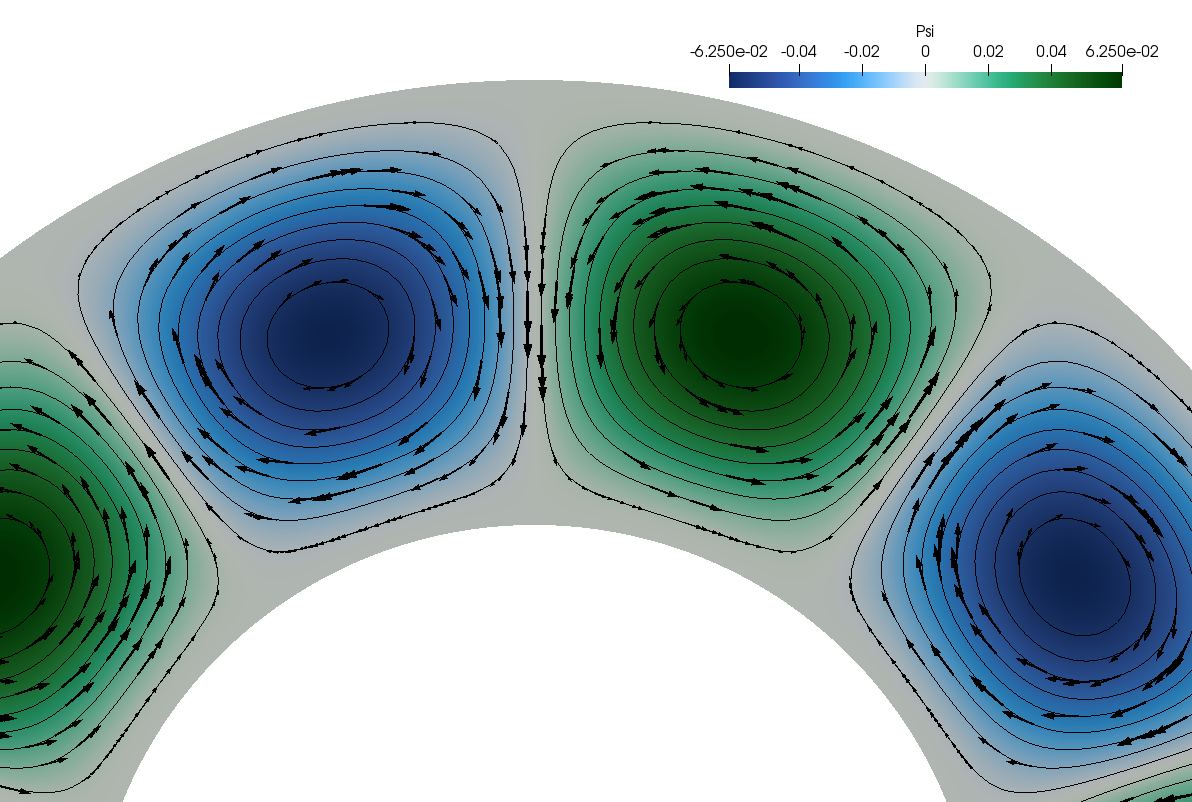
\includegraphics[width=7.3cm]{python_codes/fieldstone_35/results/iso_k5}
\end{center}







